\section{서론}
\label{sec:introduction}

종단 간(end-to-end, E2E) 자율주행은 카메라 영상과 자차 상태를 입력으로 받아 미래 궤적이나 제어 명령을 직접 예측한다 \cite{hu2023uniad,jiang2023vad}. 최근 비전-언어 모델(vision-language model, VLM)은 자연어 추론을 결합하여 장면에서 인식한 원인과 판단, 행동을 연결한다 \cite{sima2024drivelm,tian2024drivevlm}. Alpamayo-R1은 인과 연쇄(Chain-of-Causation, CoC)와 궤적을 함께 예측하는 대표적인 모델이다 \cite{wang2025alpamayo}. CoC는 "전방 차량 때문에 감속한다" 또는 "보행자에게 양보한다"처럼 특정 행동이 필요한 이유를 설명하므로, 궤적만 모방하는 학습보다 풍부한 학습 신호를 제공할 수 있다.

그러나 CoC가 행동의 이유와 목표를 설명하더라도 허용 가능한 궤적이 하나로 정해지는 것은 아니다. 예를 들어 "보행자에게 양보한 뒤 진행한다"는 요구사항만으로는 정지선을 넘지 않아야 하는지, 어느 정도의 감속도와 가가속도(jerk)를 허용할지, 상충 구역이 얼마나 오래 비어 있어야 출발할 수 있는지가 정해지지 않는다. 따라서 같은 목표를 달성하는 궤적 중에도 현재 실행 조건을 위반하는 궤적이 있을 수 있다. 반대로 지나치게 보수적인 궤적은 조건을 만족하더라도 불필요하게 진행을 멈출 수 있다.

\revtwo{여기서 기존 연구의 두 흐름 사이에 공백이 생긴다. Driving VLM과 CoC 연구는 장면의 원인, 행동의 이유 및 목표를 언어로 설명하지만, 동일한 목표를 달성하는 후보들의 허용 경계를 바꾸어 모델의 선택이 함께 바뀌는지를 직접 평가하지 않았다. 반면 형식 검증기와 실행시간 감시기는 주어진 수치 제약을 정밀하게 검사하지만, 자연어 가드가 VLM의 학습 입력으로 사용되고 그 의미가 후보 선택에 반영되는지는 다루지 않는다. 따라서 필요한 것은 기존 CoC를 대체하는 새 계획기가 아니라, 행동 목표와 실행 허용조건을 함께 제시하고 가드 변화에 대한 모델의 반응을 분리해 측정하며 그 선택을 외부 규칙으로 재검사하는 인터페이스다.}

본 논문은 기존 CoC가 일반적으로 잘못되었거나 위험하다고 주장하지 않는다. 대신 행동 목표를 설명하는 CoC에 실행 조건을 추가한 \sccoc{}를 제안한다. 요구사항은 무엇을 달성해야 하는지를 나타내고, 실행 가드는 언제 행동을 허용ㆍ금지ㆍ해제할지와 항상 지켜야 할 경계를 명시한다. 예를 들어 보행자 양보 요구사항에 "정지선을 넘지 않는다", "감속도와 가가속도의 상한을 지킨다", "상충 구역이 일정 시간 연속으로 비어 있을 때만 출발한다"는 가드를 추가할 수 있다.

\begin{figure*}[!t]
\centering
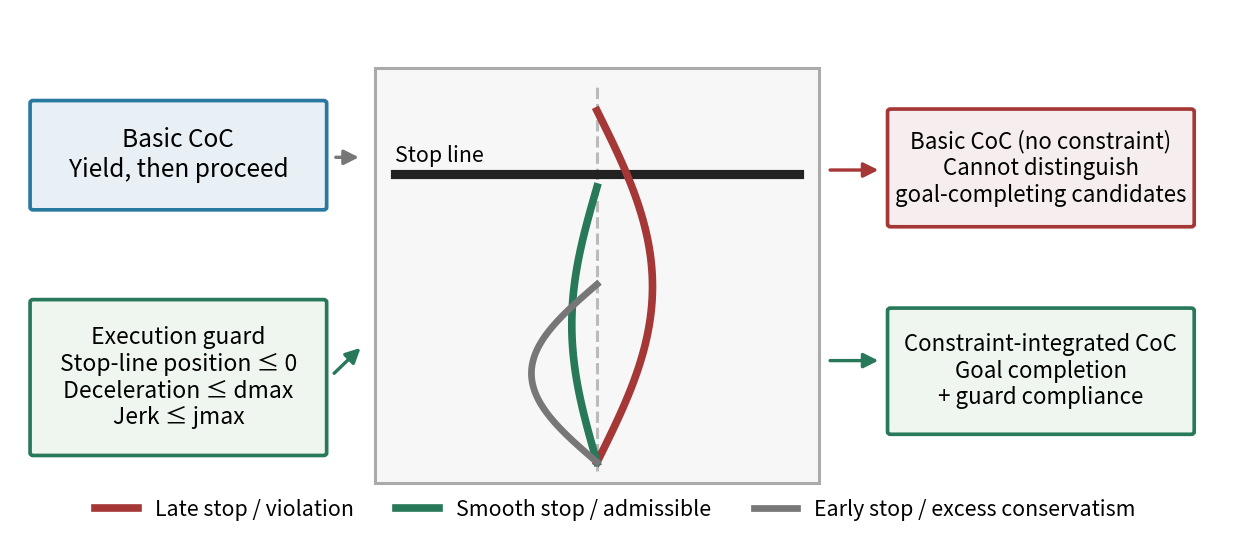
\includegraphics[width=0.98\textwidth]{../latex-kiee-review-2022/figures/fig01_concept.png}
\bifigcaption{기본 CoC와 제약 통합 CoC의 선택 기준 차이. 세 후보는 모두 `보행자에게 양보한 뒤 진행'이라는 목표와 관련되지만, 빨간 궤적은 정지선ㆍ동역학 제약을 위반하고 회색 궤적은 허용되지만 지나치게 보수적이다. 기본 CoC만으로는 두 실행 품질을 구별하기 어렵고, 제약 통합 CoC는 목표를 완료하면서 제약을 지키는 녹색 후보를 선택할 기준을 제공한다.}{Difference between basic CoC and constraint-integrated CoC: the latter distinguishes violating, overly conservative, and admissible goal-completing candidates.}
\label{fig:concept}
\end{figure*}

그림~\ref{fig:concept}은 동일한 "양보 후 진행" 목표를 달성하는 세 궤적 후보를 비교한다. 빨간색 궤적은 정지선이나 감속도ㆍ가가속도 제한을 위반하고, 회색 궤적은 필요 이상으로 일찍 정지하여 진행성을 잃는다. 반면 녹색 궤적은 행동 목표를 달성하면서 실행 가드도 만족한다. 요구사항만 포함한 CoC는 이 후보들을 명확히 구분하기 어렵지만, Safety-Constrained CoC는 목표를 유지하면서 허용 가능한 궤적을 선택할 기준을 제공한다.

제안한 가드가 궤적 선택에 실제로 영향을 주는지 확인하기 위해 같은 장면, 같은 행동 목표 및 같은 궤적 후보를 사용하되 실행 조건만 다른 두 문제를 한 쌍으로 구성한다. 이를 쌍대 계약(paired-contract) 벤치마크라 한다. 한 문제는 더 자유로운 행동을 허용하고 다른 문제는 실행 조건을 더 엄격하게 적용하므로, 두 문제에서 선택해야 할 궤적이 달라진다. 따라서 장면만 외운 모델은 두 문제를 모두 맞힐 수 없으며, 제시된 가드를 읽고 판단해야 한다. 정적 과제에서는 모든 후보가 기본 행동 목표를 달성하도록 구성하였다. 시간 과제에서는 서로 경쟁하는 진입 후보들이 목표를 달성하고, 계속 정지하는 후보는 낮은 위반률만을 노리는 교착 대조군으로 남겼다.

본 논문의 연구 질문은 다음과 같다.
\begin{enumerate}
    \item \textbf{RQ1 효과:} \sccoc{}는 요구사항만 포함한 CoC보다 가드를 위반하는 궤적의 선택을 줄이는가?
    \item \textbf{RQ2 목표 보존:} 가드 위반의 감소가 항상 정지하거나 교착되는 방식이 아니라, 행동 목표를 완료하면서 나타나는가?
    \item \textbf{RQ3 적용 범위:} 이러한 효과가 정적 후보 선택, 시간에 따른 유지ㆍ해제, 정지 및 차선 변경 상황에서도 반복되는가?
    \item \textbf{RQ4 입력 변화 강건성:} 동일 의미 문장 변형, 학습에 없던 수치, 부정ㆍ금지 표현, 경계 등호 및 단위 변환에서도 효과가 유지되는가?
\end{enumerate}

본 논문의 기여는 다음과 같다.
\begin{enumerate}
    \item 행동의 이유와 목표를 설명하는 CoC에 실행 가드를 결합한 \sccoc{}를 제안한다.
    \item 동일한 장면에서 실행 조건만 바꾸는 쌍대 계약 평가와, 행동 목표는 달성하지만 가드를 위반하는 반례 구성 방법을 제시한다.
    \item 가드 위반, 목표 완료, 교착, 과도한 보수성 및 계약 쌍의 정확도를 함께 측정하는 평가 체계를 구성한다.
    \item 한 난수 초기값(seed)의 정적 후보 실험과 데이터 생성 및 학습 난수를 함께 바꾼 세 난수 초기값의 시간ㆍ다중 주행 과제를 통해, 소형 VLM의 가드 기반 후보 선택이 표준 평가에서는 학습되지만 미관측 시간값 평가에서는 크게 약화됨을 함께 보인다.
    \item 저장한 세 난수 초기값의 어댑터를 원본ㆍ단색ㆍ충돌 영상에서 다시 평가하여, 표준 시간 과제는 영상에 의존하지만 다중 주행의 표준ㆍ미관측 수치 평가는 수치가 적힌 문장만으로 해결됨을 분리한다.
    \item 단일 장면 Alpamayo-R1 진단과 별도 소형 신경망 폐루프 실험을 보조 증거로 제시하여, 입력 문장에 대한 반응, 학습된 후보 선택 및 실행 중 강제 적용을 서로 구분한다.
\end{enumerate}

\revtwo{제안 방법의 장점은 네 가지다. 첫째, 기존 CoC의 설명 구조를 유지하면서 누락되기 쉬운 허용ㆍ금지ㆍ해제 조건을 자연어로 명시할 수 있다. 둘째, 쌍대 계약은 장면과 행동 목표를 고정하므로 높은 정확도가 장면 암기인지 가드에 따른 선택 전환인지 구분한다. 셋째, 가드 위반률과 목표 완료ㆍ교착ㆍ과도한 보수성을 함께 측정하여 항상 정지하는 해법을 성공으로 세지 않는다. 넷째, 후보 선택과 수치 판정을 분리하므로 같은 가드를 모델 외부 결정적 검증기 또는 실행 차단장치로 연결할 수 있다. 이 장점들은 합성 후보 선택의 해석 가능성과 진단 가능성에 관한 것이며 실제 차량의 안전 보장을 뜻하지 않는다.}

본 연구는 합성 이미지와 수치 설명으로 제시된 궤적 후보를 사용하여 소형 VLM의 학습 가능성을 평가한다. 영상 절제에서 표준 시간 과제는 여러 시점을 이어 붙인 연속 장면 영상에 의존했지만, 다중 주행의 표준ㆍ미관측 수치 평가는 단색 영상과 반대 행동 영상에서도 성능이 유지되어 문장 정보만으로 풀 수 있었다. 따라서 합성 영상의 시간 정보 사용은 확인했으나 실제 도로의 시각적 근거화를 입증하지는 않는다. 실험에 사용한 정지선, 최소 간격, 속도 및 대기시간 가드는 제안한 표현과 평가 방법을 시험하기 위해 연구자가 미리 정한 조건이다. 실제 도로의 CoC로부터 어떤 제약 조건을 선택하고 그 수치와 해제 조건을 어떻게 도출할 것인지도 본 논문에서 제시하거나 검증하지 않는다. 따라서 실제 차량의 충돌 감소, Alpamayo-R1을 학습한 뒤의 성능 향상 또는 완전한 도로 안전 명세를 입증하지는 않는다.

\revtwo{이후 논문의 흐름은 다음과 같다. 2장은 driving VLM과 실행 검증 연구 사이의 공백을 정리하고, 3장은 행동 목표와 실행 가드를 분리하여 선택 문제를 정의한다. 4장은 Safety-Constrained CoC 입력, 쌍대 계약 및 모델 외부 검증 지표를 제시한다. 5장은 정적ㆍ시간ㆍ다중 주행 후보 선택과 별도 폐루프 보조 실험을 순서대로 보고한다. 6장은 결과의 의미와 학습된 가드 준수ㆍ실제 실행 안전의 경계를 논의하고, 7장은 결론과 후속 과제를 정리한다.}
